\documentclass[a4paper]{article}
\usepackage[utf8]{inputenc}
\usepackage[english]{babel}

\usepackage{pdfpages}
\usepackage{amsmath}
\numberwithin{equation}{section}
\usepackage{amsfonts}
\usepackage{amssymb}
\usepackage{mathtools}
\usepackage{graphicx}
\usepackage{pdfpages}
\usepackage{enumitem}
\usepackage{paralist}

\newcommand{\ie}{\textit{i.e.,} }
\newcommand{\eg}{\textit{e.g.,} }

\usepackage[style=authoryear, backend=bibtex,maxnames=2,sorting=ydnt]{biblatex}
\usepackage[colorlinks=true, linkcolor=red, citecolor=blue]{hyperref}
\renewcommand*{\mkbibnamefamily}[1]{\textsc{#1}}
\addbibresource{refs.bib} %Import the bibliography file

\usepackage{csquotes}

\usepackage[font=sf,labelfont={sf,bf},]{caption}
\usepackage[outercaption]{sidecap}
\captionsetup[figure]{format=plain}
\captionsetup[table]{format=plain}
\DeclareCaptionLabelSeparator{bar}{ | }
\captionsetup{
	labelsep=bar
}

\usepackage{fontawesome}




\begin{document}
\title{The finite volume method for conservative nonlinear hyperbolic systems: the Saint-Venant equations}
\date{\today}
	\author{\texttt{mad max}}
	\maketitle
	\nocite{*}
	
	\section*{Abstract}
	
	\section{Generalities}
	This document is heavily inspired by the lecture notes of \cite{Lagree2022}
	\subsection{Saint-Venant (SV) or the shallow water (SW) equations}
	Adhémar Jean-Claude Barré de Saint-Venant proposed 150 years ago the following system of nonlinear hyberbolic partial differential equations (PDE's) for a one-dimensional steady fluid motion. They are derived from depth-integrating the Navier-Stokes equations under simplifying assumptions\footnote{One of these is the hydrostatic pressure distribution, \ie $\partial_zp + \rho g = 0$ (see \cite[pp. 22]{castro2019}). This yields a bottom pressure $p|_{z}=\rho g h$, \ie the weight of the water column above, and a linear pressure distribution.} (see \cite[pp. 35]{toro2013}). Such system reads as
	\begin{align}
		\label{StVenant}
		\begin{cases}
			\partial_t h + \partial_xQ = 0 \\
			\partial_t Q + \partial_x \left( \Gamma \frac{Q^2}{h}+g\frac{h^2}{2} \right) = -gh\partial_{x}z-\frac{\tau}{\rho} ,
		\end{cases}
	\end{align}
	with $h(x,t)$ the water height, $Q(x,t)=h(x,t)u(x,t)$ the flow discharge, $u(x,t)$ the depth-averageg velocity, $\Gamma$ a shape factor (Boussinesq coefficient), $\tau$ the basal shear resistance law (given by $Q$ and oriented as $-Q/|Q|$), $z(x,t)$ the (bed) topography and $g$ the gravity. The reader should keep in mind that other formulations exist in the litterature for more specific applications\footnote{
	As an example, for unsteady open channel flow \parencite{kerger2011,hodges2019}, the system  \ref{StVenant} is often expressed (after area-integrating of the Navier-Stokes equations) as
	\begin{align}
	\label{StVenantOpenChannel}
	&\begin{cases}
		\partial_t A + \partial_xQ = 0 \\
		\partial_t Q + \partial_x \left(  \frac{Q^2}{A}+gI_1 \right) = gA(S_0-S_f)+gI_2,
	\end{cases}
	 \end{align}
 	completed by the following
	 \begin{align}
	 I_1(h)=\int_{-h_b}^{h_{fs}}(h-\xi)l(x,\xi)\mathrm{d}\xi \,\,,\,\, I_2(h)=\int_{-h_b}^{h_{fs}}(h-\xi) \partial_x l(x,\xi) \mathrm{d}\xi
	\end{align}	
	where $A$ is the flow area, $Q=Au$ is the flow discharge, $S_0$ is the river bed slope, $S_f$ is the friction term resulting from the resistance law, $h$ is the water height, $l$ is the free-surface width, $h_{fs}$ is the free surface elevation and $h_b$ is the bottom elevation. 
	
	The friction term $S_f$ is assumed to be given by the Manning-Strickler relation, which reads
	\begin{align}
		S_f = \frac{Q|Q|}{A^2K^2R_h^{4/3}},
	\end{align}
	where $K$ is the Strickler coefficient and $R_h$ is the hydraulic radius.
	}, \eg numerical solutions to channel routing for hydraulic application, see \texttt{RS MINERVE} (\url{https://crealp.ch/rs-minerve/}).
	\subsubsection{Closure of the system}
	For rivers and streams, one can choose the following expressions for $\Gamma$ and $\tau$
	\begin{align}
		\Gamma = 1 \,\,\,\, \mathrm{and} \,\,\,\, \tau = \rho c |Q| \frac{Q}{h^{\beta}},
	\end{align}
	where $\Gamma=1$ because a sufficiently smooth bottom is assumed and $\beta=2$ (the Chezy or Darcy Weissbach law) or $\beta=7/3$ (the Manning-Strickler law).
	
	However, other expressions can be defined. As an example, for complex flows such as glacier flows (the Glen law gives $n=1/3$) or mud flows ($0.1<n<0.4$), we have
	\begin{align}
		\Gamma = \frac{2(1+2n)}{2+3n} \,\,\,\, \mathrm{and} \,\,\,\, \tau = c_n\mu_n \left( \frac{Q}{h^2} \right)^n \frac{|Q|}{Q},
	\end{align}
	where $\mu_n$ is the friction coefficient. For the snow, the Voellmy law can be adopted and reads
	\begin{align}
	\Gamma = 1 \,\,\,\, \mathrm{and} \,\,\,\, \tau = \rho g h \left( \mu_0 + \frac{1}{\xi}\frac{Q^2}{h^3} \right) \frac{|Q|}{Q},
	\end{align}
	where, typically, $\mu_0=0.2$ and $\xi=500$ m$\cdot$s$^{-1}$. 

	\subsection{Compact conservative form of the system}
	Let us rewrite the system of hyperbolic PDE's \ref{StVenant} as a \underline{compact} and \underline{conservative} system of equations\footnote{Assuming $\Gamma=1$, which is widely accepted in the litterature.} in \underline{differential form}, such as 
	\begin{align}
		\label{StVenantCompact}
		\partial_t \mathbf{U}+\partial_x \mathbf{F(U)} = \mathbf{S(U)},
%		\partial_t \boldsymbol{u}+\partial_x \boldsymbol{f}(\boldsymbol{u}) = \boldsymbol{S}(\boldsymbol{u}),		
	\end{align}
	where $\mathbf{U}$ is the vector of conservative variables, $\mathbf{F(U)}$ is the flux function vector and $\mathbf{S(U)}$ the source term vector
		\begin{align}
		\mathbf{U} = 
		\begin{bmatrix}
			h \\
			Q
		\end{bmatrix}, \,\,\,
		\mathbf{F(U)} = 
		\begin{bmatrix}
			Q \\
			\frac{Q^2}{h}+g\frac{h^2}{2}
		\end{bmatrix}, \,\,\,	
		\mathbf{S(U)} = 
		\begin{bmatrix}
			0 \\
			-gh\partial_{x}z-\frac{\tau}{\rho}
		\end{bmatrix}.
	\end{align}

	\subsubsection{The Jacobian of the flux function}
	Let us consider $\mathbf{S(U)}:=\mathbf{0}$ in \ref{StVenantCompact} and then derive the flux function vector $\mathbf{F(U)}$ using the chain rule. Then, one obtains that $\partial_x\mathbf{F(U)}=\partial_{\mathbf{U}}\mathbf{F(U)}\cdot\partial_x\mathbf{U}$, which yields to
	\begin{align}
		\partial_x\mathbf{F(U)} &= 
		\begin{bmatrix}
			\partial_hQ & \partial_QQ \\
			\partial_h (\frac{Q^2}{h}+g\frac{h^2}{2}) & \partial_Q (\frac{Q^2}{h}+g\frac{h^2}{2}) 
		\end{bmatrix}\cdot
		\partial_x		
		\begin{bmatrix}
			h \\
			Q 
		\end{bmatrix},\\
		\partial_x\mathbf{F(U)} &= 
		\begin{bmatrix}
			0 & 1 \\
			gh-\frac{Q^2}{h^2} & \frac{2Q}{h}
		\end{bmatrix}\cdot
		\partial_x		
		\begin{bmatrix}
			h \\
			Q 
		\end{bmatrix},\\ 
		\partial_x\mathbf{F(U)} &= 
		\begin{bmatrix}
			0 & 1 \\
			gh-u^2 & 2u
		\end{bmatrix}\cdot
		\partial_x		
		\begin{bmatrix}
			h \\
			Q 
		\end{bmatrix},\\ 
		\partial_x\mathbf{F(U)} &= \mathbf{J(U)}\partial_x\mathbf{U}.
	\end{align}

	Now, the system \ref{StVenantCompact} can be rewritten with such alternative definition of the flux vector function, such as
	\begin{align}
		\partial_t \mathbf{U}+\mathbf{J(U)}\partial_x\mathbf{U} = \mathbf{0},
	\end{align}
	
	The Jacobian\footnote{In the classical textbooks \cite{leveque_2002,toro2013} about hyperbolic systems, the Jacobian of the flux function vector is often referred as $\mathbf{A}\equiv\mathbf{A}(\mathbf{U})$.} of the flux function  $\mathbf{J(U)}\equiv\partial_{\mathbf{U}}\mathbf{F(U)}$ has two eigenvalues, \ie $\lambda^{(1,2)}_{\mp}$, and two eigenvectors, \ie $\boldsymbol{\lambda}^{(1,2)}$. They can be found by solving
	\begin{align}
		|\mathbf{J(U)}-\lambda\mathbf{I}|=\mathrm{det}(\mathbf{J(U)}-\lambda\mathbf{I})=0,
	\end{align}
	with the solutions $\lambda^{\mp}_{(1,2)} = u \mp c$. These eigenvalues will be further used to reconstruct or estimate \underline{numerical fluxes}\footnote{It should not be understood as physical fluxes.} at the interface between two control volumes\footnote{Actually, this is the key point of any finite volume approximation. Estimating or approximating these inter-cell numerical fluxes at the interface is of utmost importance and is a real crux of the method. Particularly, finding an accurate solution to the local Riemann problem is central in every finite volume approximations.}, \ie where \underline{a local Riemann problem} exists (we will come back later on this concern in  \ref{riemann_problem_section}). The eigenvalues $\lambda^{\mp}_{(1,2)}$ are given by
	\begin{align}
		\lambda_{(1)}^{-} = \frac{Q}{h} - \sqrt{gh} \,\,\,\, \mathrm{and} \,\,\,\, \lambda_{(2)}^{+} = \frac{Q}{h} + \sqrt{gh},
	\end{align}
	whereas the eigenvector are expressed as
	\begin{align}
		\boldsymbol{\lambda}^{(1)}=		
		\begin{bmatrix}
			-c/h \\
			1 
		\end{bmatrix}
		\,\,\,\, \mathrm{and} \,\,\,\,
		\boldsymbol{\lambda}^{(2)}=		
		\begin{bmatrix}
			c/h \\
			1 
		\end{bmatrix},
	\end{align}
	where $c=\sqrt{gh}$ is the wave propagation speed or \textit{celerity}, hence denoted by $c$. It could be think of as a \textit{gravity} wavespeed \parencite{kerger2011}.
	
	Such system is called  \textit{hyperbolic}\footnote{In general, a system \enquote{is said to be hyperbolic at a point $(x,t)$ if $\mathbf{A}$ has $m$ real eigenvalues $\lambda_1,...,\lambda_m$ and a corresponding set of $m$ linearly independent right eigenvectors $\mathbf{K}^{(1)} ,..., \mathbf{K}^{(m)}$. The system is said to be strictly hyperbolic if the eigenvalues $\lambda_i$ are all distinct} \parencite[see pp. 45, chap. 2.1 Quasi-Linear Equations: Basic Concepts]{toro2013}.} since the Jacobian $\mathbf{J(U)}$ is i) diagonalizable and, ii) has real eigenvalues  \parencite[see pp. 31, chap. 2.9 Hyperbolicity of Linear Systems]{leveque_2002}. 
		
	\newpage	
	\section{Numerical resolution: the finite volume approximation}
	As stated in \cite[pp. 64]{leveque_2002}, finite volume methods \enquote{are closely related to finite difference methods, and a finite volume method can often be interpreted directly as a finite difference approximation to the differential equation. However, finite volume methods are derived on the basis of the \underline{integral form} of the conservation law, a starting point that turns out to have many advantages}.
		\begin{figure}[htbp]
		\centering
		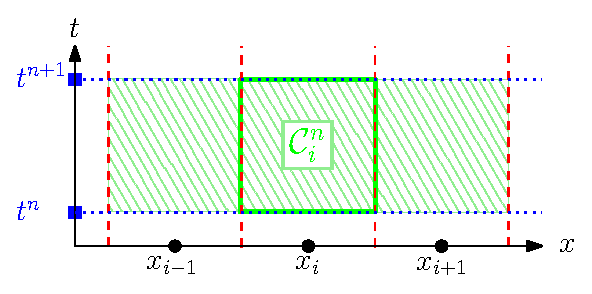
\includegraphics[scale=0.75]{imgs/fvdisc_spacetime.eps}
		\caption{Typical finite volume discretization in the $x-t$ plane, with a volume control $\mathcal{C}_i$.}
		\label{fv_spacetime}
	\end{figure}

	In the following, we will see how to express the differential form of the hyperbolic system \ref{StVenantCompact} into an integral form of such conservative system.
	\subsection{Finite volume discretization (space and time)}
	The first step for any numerical approximation is to discretize the continuous domain (in space and time). 
	
	Let us consider a \textit{uniform} discretization of the continuous domain $[x_L,x_R]$ into a regular grid composed of discrete points. These are denoted as
	\begin{align}
		x_i=x_L+(i+1/2)\Delta x \,\,\,\, \mathrm{for}\,\,\,\, i=0,...,n,
	\end{align}
	with $\Delta x = \frac{x_R-x_L}{n+1}$. Let us also define midpoint or edge values
	 \begin{align}
	  	x_{i-\frac{1}{2}}=x_i-\Delta x /2 \,\,\,\, \mathrm{for}\,\,\,\, i=0,...,n+1.
	 \end{align}
	
	These values define the \textit{control volumes} or cells or elements such that we have the following definition
	\begin{align}
		\mathcal{C}_i = [x_{i-\frac{1}{2}},x_{i+\frac{1}{2}}],
	\end{align} 
	and they are naturally centered at the $x_i$ location. Adding a temporal discretization for a time interval $t\in[t_0,t]$, and, one obtain the following discretization for a given control volume $\mathcal{C}_i=[x_{i-\frac{1}{2}},x_{i+\frac{1}{2}}]\times[t_{n},t_{n+1}]$ (see Figs. \ref{fv_spacetime} \& \ref{fv_discretization}).
	\begin{figure}[htbp]
		\centering
		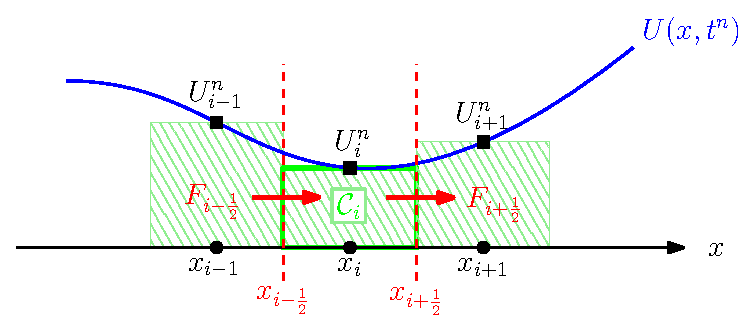
\includegraphics[scale=0.75]{imgs/fvmdiscr.eps}
		\caption{Finite volume discretization (only spatial discretizazion is shown here), inspired from \cite{Lagree2022}. The continuous solution $U^n$ is discretized into a piece-wise constant distribution \parencite{godunov1959} of data $U_i^n$ at the center of the control volume $\mathcal{C}_i$, where $n$ indicates the temporal discretization and $i$ the spatial discretization.}
		\label{fv_discretization}
	\end{figure}

	
	\subsection{Integral form of conservative hyperbolic systems}
	Starting with the finite volume discretization, \ie $\mathcal{C}_i = [x_{i-\frac{1}{2}},x_{i+\frac{1}{2}}]$, the value $\mathbf{U}_i^n$ will approximate the average value (or the cell average\footnote{The reader should observe that one can choose a piece-wise constant approximation to $\mathbf{U}_i^n$, \ie $\mathbf{U}_i^n \approx \mathrm{cst}$ in the control volume $\mathcal{C}_i$.}) over the $i$th interval at a time $t_n$, such as
	\begin{align}
		\label{cell_average}
		\mathbf{U}_i \approx \frac{1}{\Delta x} \int_{x_{i-\frac{1}{2}}}^{x_{i+\frac{1}{2}}} \mathbf{U}(x,t) \mathrm{d}x \equiv \frac{1}{\Delta x} \int_{\mathcal{C}_i} \mathbf{U}(x,t) \mathrm{d}x.
	\end{align}

	After defining a cell-average description of $\mathbf{U}(x,t)$ over a control volume $\mathcal{C}_i$, let us have a look to the integral form of the conservative system. The integral form of the conservative system \ref{StVenantCompact}, now reads as
	\begin{align}
	\int_{\mathcal{T}}\int_{\mathcal{C}_i} [\partial_t \mathbf{U}(x,t)+\partial_x \mathbf{F}(\mathbf{U}(x,t))] \mathrm{d}x \mathrm{d}t = \int_{\mathcal{T}}\int_{\mathcal{C}_i} \mathbf{S(U)} \mathrm{d}x \mathrm{d}t,
	\end{align}	
	where $\mathcal{T}=[t^n,t^{n+1}]$ and $\mathcal{C}=[x_{i-\frac{1}{2}},x_{i+\frac{1}{2}}]$, with $t^{n+1}=t^n+\Delta t$, which generates, after integration and when considering $\mathbf{S(U)}:=\mathbf{0}$, 
	\begin{align}
		\frac{\mathrm{d}}{\mathrm{d}t} \int_{\mathcal{C}_i} \mathbf{U}(x,t) \mathrm{d}x = \mathbf{F}(\mathbf{U}(x_{i-\frac{1}{2}},t)) - \mathbf{F}(\mathbf{U}(x_{i+\frac{1}{2}},t)).
	\end{align}
	Then, integrating in time from $t_n$ to $t_{n+1}$, rearranging and dividing by $\Delta x$ yields to a general numerical scheme of the form
	\begin{align}
		\label{conservative_numerical_scheme}
		\mathbf{U}_i^{n+1} = \mathbf{U}_i^{n} - \frac{\Delta t}{\Delta x}( \mathbf{F}_{i+\frac{1}{2}}^n - \mathbf{F}_{i-\frac{1}{2}}^n ),
	\end{align}
	where $\mathbf{F}_{i\pm\frac{1}{2}}^n$ is some approximation of the average numerical fluxes at the inter-cells $x=x_{i\pm\frac{1}{2}}$, as
	\begin{align}
		\label{numerical_intercell_fluxes}
		\mathbf{F}_{i\pm\frac{1}{2}}^n \approx \frac{1}{\Delta t} \int_{t_n}^{t_{n+1}} \mathbf{F}(\mathbf{U}(x_{i\pm\frac{1}{2}},t))\mathrm{d}t.
	\end{align}

	The general concern of any finite volume method is to find a good enough approximation of \ref{numerical_intercell_fluxes} and, we will see in the following different approximations of these inter-cell numerical fluxes to solve for the discrete conservative hyperbolic system in integral form.

	\subsection{Solution strategy (with or without a source term)}
	To solve numerically for the system of hyperbolic partial differential equations (PDE's, see \ref{StVenantCompact}) with initial conditions (IC's) of considering a source term, a \underline{splitting scheme} (or approach) \parencite{toro2001,castro2019} can be used. The general problem is to determine the conservative variables vector $\mathbf{U}$ at time $t^{n+1}$, considering the effect of the source term(s), and this reads as 
	\begin{align}
		\label{PDE_system_to_be_soved}
		\begin{rcases}
			\text{PDE's} &\partial_t \mathbf{U}+\partial_x \mathbf{F(U)} = \mathbf{S(U)}\\
			\text{IC's} &\mathbf{U}(x,t)=\mathbf{U}_i^n
		\end{rcases} 
		\Rightarrow \mathbf{U}_i^{n+1}(x_i,t^{n+1}).
	\end{align}
	The splitting approach solves the general problem \ref{PDE_system_to_be_soved} in two consecutive steps, which are given in the following.
	
	(\textit{Step 1}) Let us solve the homogeneous part of \ref{PDE_system_to_be_soved} using an appropriate numerical scheme, \ie a Godunov-type scheme, such as
	\begin{align}
		\begin{rcases}
			\text{PDE's} &\partial_t \mathbf{U}+\partial_x \mathbf{F(U)} = \mathbf{0}\\
			\text{IC's} &\mathbf{U}(x,t)=\mathbf{U}_i^n
		\end{rcases} 
		\Rightarrow \mathbf{U}_i^{\mathrm{adv}}(x_i,t^{n+1}),
	\end{align}
	where the temporary solution $\mathbf{U}_i^{\mathrm{adv}}(x_i,t^{n+1})$ accounts for the effects of advection. This step can be regarded as a predictor step (or transient) to approximate a solution due to advective transport, outlooking the effects of any source terms. The transient  solution due to advection (within a proper conservative numerical scheme) is given by
	\begin{align}
		\mathbf{U}_i^{\mathrm{adv}} = \mathbf{U}_i^{n} - \frac{\Delta t}{\Delta x}( \mathbf{F}_{i+\frac{1}{2}}^n - \mathbf{F}_{i-\frac{1}{2}}^n ),
	\end{align}
	and, if initially considering no source terms, \ie $\mathbf{S(U)}:=\mathbf{0}$, then the solution procedure is over and one has $\mathbf{U}_i^{n+1}(x_i,t^{n+1}):=\mathbf{U}_i^{\mathrm{adv}}$. 
	
	(\textit{Step 2}) Update (or correct) the transient solution including effects of the source terms, such as 
	\begin{align}
		\label{ODE_system_to_be_soved}
		\begin{rcases}
			\text{ODE's} &\partial_t \mathbf{U} = \mathbf{S(U)}\\
			\text{IC's} &\mathbf{U}(x,t)=\mathbf{U}_i^{\mathrm{adv}}
		\end{rcases} 
		\Rightarrow \mathbf{U}_i^{n+1}(x_i,t^{n+1}),
	\end{align}
	which can be solved with a variety of ODE solvers. This step can be regarded as a correction step, as opposed to the predictor step in the first stage of the solution strategy. A \underline{first-order forward Euler} scheme is a fair choice, and it reads 
	\begin{align}
		\mathbf{U}_i^{n+1} = \mathbf{U}_i^{\mathrm{adv}} + \Delta t \mathbf{S(U)},
	\end{align}
	but a better approximation is given by 
	\begin{align}
		\mathbf{U}_i^{n+1} = \mathbf{U}_i^{\mathrm{adv}} + \Delta t \mathbf{S(\mathbf{U}_i^{\mathrm{adv}})},
	\end{align}
	where the source terms take into account the effects of advection over the conservative variable vector.
	
	Other schemes exist, such as \underline{first-order backward Euler} scheme and the \underline{second-order or third-order TVD Runge-Kutta} scheme to name a few. 

	\subsection{The Riemann problem}\label{riemann_problem_section}
	A Riemann problem\footnote{For a clear discussion of a Riemann problem, one can refer to the classical textbook of \cite{toro2013}. In particular, a complete description is given in \cite[see pp. 49, chap. 2.2 The Linear Advection Equation]{toro2013}} is a specific initial value problem (IVP) composed of a conservation equation together with piece-wise constant data reconstruction \parencite{godunov1959}, which has a single discontinuity in the domain being considered. It is a widely encountered problem in computational fluid dynamics, especially when a piece-wise constant distribution is assumed (\eg the Godunov-type methods, see \cite{guinot2012,toro2013}). 
	\begin{figure}[htbp]
		\centering
		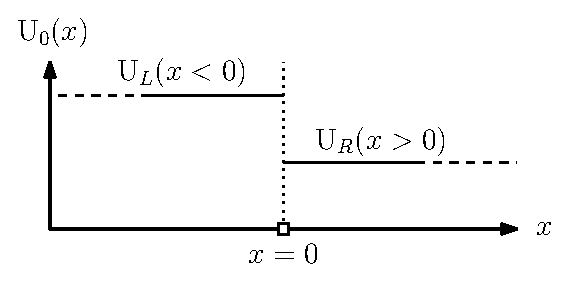
\includegraphics[scale=0.75]{imgs/riemann_problem.eps}
		\caption{Sketch of the initial data (constant distribution with a single discontinuity) for the Riemann problem. The initial data consist of two constant states $\mathrm{U}_{L,R}$ separated by a discontinuity located at $x = 0$.}
		\label{riemann_problem_scheme}
	\end{figure}
	
	The local Riemann problem for the Saint-Venant equations under a piece-wise constant distribution (see \ref{godunov_method} and Fig. \ref{fv_discretization}) is formally defined as an initial-value problem and reads
	\begin{align}
	\begin{rcases}
		\label{riemann_problem}
		&\partial_t \mathbf{U}+\partial_x \mathbf{F(U)} = \mathbf{0},\\
		&\mathbf{U}(x,0)=\mathbf{U}_0(x)=
		\begin{cases}
			\mathbf{U}_L  &\,\,\,\, \mathrm{for} \,\,\,\, x<0,\\
			\mathbf{U}_R  &\,\,\,\, \mathrm{for} \,\,\,\, x>0,\\
		\end{cases}
	\end{rcases} 
	\end{align}
	where the discontinuity initially located at $x=0$ at time $t=0$ is moving throughout time. 
	
	A Riemann solver aims at finding the solution (approximate or exact) to the local Riemann problem, which can be further used to determine numerical fluxes. The solution to the local Riemann problem $\mathbf{U}(x,t)$ subject to \ref{riemann_problem} is to be determined from
	\begin{align}
		 \partial_t \mathbf{U}+\partial_x\mathbf{F} = \mathbf{0}.
	\end{align}
 
	We will now refer to the Riemann problem as $\mathcal{R}(\mathbf{U}_L,\mathbf{U}_R)$. The solution can be exactly calculated (see \cite{castro2019,toro2013,leveque_2002}), but we will see, in the following, numerical techniques to approximate the solution to the Riemann problem  $\mathcal{R}(\mathbf{U}_L,\mathbf{U}_R)$.

	\subsection{Godunov-type methods for the local Riemann problems}
	\subsubsection{The Godunov method}\label{godunov_method}
	The method was first proposed by \cite{godunov1959} and it is a first-order scheme \parencite{toro2013}. The numerical fluxes need to be calculated at the interface between two control volumes $\mathcal{C}_{i}$ and $\mathcal{C}_{i+1}$ to satisfy a conservative numerical scheme. Exploiting the definition of cell average (see \ref{cell_average}) and constucting a piece-wise constant distribution, a local Riemann problem arises at each interface between adjacent cells, resulting in a single discontinuity. Each local Riemann problem $\mathcal{R
	}(\mathbf{U}_{i},\mathbf{U}_{i+1})$ is defined as
	\begin{align}
		\begin{rcases}
			&\partial_t \mathbf{U}+\partial_x \mathbf{F(U)} = \mathbf{0},\\
			&\mathbf{U}_0(x)=
			\begin{cases}
				\mathbf{U}_L  &\,\,\,\, \mathrm{for} \,\,\,\, x_{i-0}<x<x_{i+\frac{1}{2}},\\
				\mathbf{U}_R  &\,\,\,\, \mathrm{for} \,\,\,\, x_{i+\frac{1}{2}}<x<x_{i+1},\\
			\end{cases}
		\end{rcases} 
	\end{align}
	and, the inter-cell numerical fluxes $\mathbf{F}_{i+\frac{1}{2}}$ are computed using solutions of local Riemann problems. One generally expresses the \textit{Godunov} inter-cell numerical fluxes as 
	\begin{align}
		\mathbf{F}_{i\pm\frac{1}{2}}^{\mathrm{god}} = \mathbf{F}(\mathbf{U}_{i\pm\frac{1}{2}}(0)),
	\end{align}
	where $\mathbf{U}_{i\pm\frac{1}{2}}(0)$ denotes the solution of the Riemann problem $\mathcal{R}(\mathbf{U}_{i},\mathbf{U}_{i+1})$. 
	
	The implementation of the Godunov's scheme is given in the following procedure:
	\begin{compactitem}
		\item start at $t^n$ with known cell-averaged values $\mathbf{U}_i$ over the computational domain,
		\item set the boundary conditions,
		\item solve (exact or approximate) $\mathcal{R}(\mathbf{U}_{i},\mathbf{U}_{i+1})$ at inter-cell location $i+\frac{1}{2}$, and for any control volume $\mathcal{C}_i$,
		\item update $\mathbf{U}_i^n$ to $\mathbf{U}_i^{n+1}$ using \ref{conservative_numerical_scheme},
		\item repeat.
	\end{compactitem}
	
	\subsubsection{The HLL (Harten, Lax, van Leer) approximate Riemann solver}
	An approximate Riemann solver was proposed by Harten, Lax and van Leer in 1983 and was coined HLL\footnote{A more accurate method is the HLLC solver, proposed by Toro and co-workers in 1992, see \cite{toro2001,toro2019}. It considers a \textit{three-wave model} and better resolve intermediate waves at the discontinuity.} solver \parencite{harten1983} and it requires estimates for the fastest signal velocities emerging at the local Riemann problem, \ie the discontinuity. This resulted in a \textit{two-wave model}. 
	
	Formally, the approximate numerical flux is given by the following \parencite{toro2001,huang2013,toro2013,toro2019}:
	\begin{align}\label{hll_fluxes}
		\mathbf{F}_{i+\frac{1}{2}}=
		\begin{cases}
			\mathbf{F}_{L} & \text{if}\quad s_L \geq 0, \\
			\mathbf{F}^{\mathrm{hll}}=\frac{ s_R\mathbf{F}_{L}-s_L\mathbf{F}_{R}+s_Rs_L(\mathbf{U}_{R}-\mathbf{U}_{L}) }{s_R-s_L}& \text{if} \quad s_L \leq 0 \leq s_R,\\
			\mathbf{F}_{R}& \text{if}\quad s_R \leq 0,
		\end{cases} 
	\end{align}
	where a reliable estimate for the wave speeds $s_{L,R}$ at the discontinuity (considering wet-dry transition) is needed, \ie
	\begin{align}
		s_L=
\begin{cases}
u_R - 2a_R & \text{if}\quad h_L = 0, \\
\min(u_L - a_L,u_{\star} - a_{\star}) & \text{if}\quad h_L > 0, \\
\end{cases} 
	\end{align} 
and,
	\begin{align}
	s_R=
	\begin{cases}
		u_L + 2a_L & \text{if}\quad h_R = 0, \\
		\max(u_R +a_R, u_{\star} - a_{\star}) & \text{if}\quad h_R > 0, \\
	\end{cases} 
\end{align} 
where
	\begin{align}
	q_{L,R}=
	\begin{cases}
		\sqrt{\frac{1}{2}(\frac{(h_{\star}+h_{L,R})h_{\star}}{h^2_{L,R}})} = 0 & \text{if}\quad h_{\star} > h_{L,R}, \\
		1 & \text{if}\quad h_{\star} \leq h_{L,R}, \\
	\end{cases} 
\end{align}
with 
\begin{align}
	h_{\star}&=\frac{1}{g}\left(\frac{1}{2}(a_L+a_R)+\frac{1}{4}(u_L-u_R)\right)^2, \\
	u_{\star}&=\frac{1}{2}(u_L+u_R)+(a_L-a_R),\\
	a_{L,R,\star}&=\sqrt{g h_{L,R,\star}}.
\end{align}
	
	\subsubsection{The Rusanov flux}
	Another estimate for wave speed velocities is the following:
	\begin{align}
		s_L = -s^{+} \quad \text{,} \quad s_R = s^{+},
	\end{align}
	where the estimate $s^{+}=\max(|u_L|+a_L,|u_R|+a_R)$. If $s_{L,R}$ are substituted in \ref{hll_fluxes} following this maximum wave speed estimate, one obtain the Rusanov flux, \ie
	\begin{align}
		\mathbf{F}_{i\pm\frac{1}{2}}^{\mathrm{Rus}}= \frac{1}{2}(\mathbf{F}_{L}+\mathbf{F}_{R}) - \frac{1}{2}s^{+}(\mathbf{U}_{R}-\mathbf{U}_{L}).
	\end{align}

	If one selects $s^{+}=\frac{\Delta x}{\Delta t}$, this results in the Lax-Friedrich flux
	\begin{align}
	\mathbf{F}_{i\pm\frac{1}{2}}^{\mathrm{LF}}= \frac{1}{2}(\mathbf{F}_{L}+\mathbf{F}_{R}) - \frac{\Delta x}{2\Delta t}(\mathbf{U}_{R}-\mathbf{U}_{L}).
	\end{align}
	
	\subsubsection{The Courant Friedrich Levy condition (CFL)}
	To ensure numerical stability of the solution, the CFL condition requires that 
	\begin{align}
		\mathrm{max}(|\lambda_i|)\frac{\Delta t}{\Delta x} \leq 1,
	\end{align}
	and if this condition is satisfied, no characteristics waves will travel across discontinuities of neighbouring local Riemann problems. As a result, local solutions will not be influenced by waves travelling across the domain.
		
	\section{Channel routing in \texttt{RS MINERVE}}
	\subsection{Saint Venant type}
	\subsection{Muskingum-Cunge type}
	\subsection{Kinematic wave type}





	\newpage
	\printbibliography[title={References}]

\end{document}


% see overleaf works just fine !!